% CVPR 2024 Paper Template; see https://github.com/cvpr-org/author-kit

\documentclass[10pt,twocolumn,letterpaper]{article}

%%%%%%%%% PAPER TYPE  - PLEASE UPDATE FOR FINAL VERSION
\usepackage{cvpr}              % To produce the CAMERA-READY version
% \usepackage[review]{cvpr}      % To produce the REVIEW version
% \usepackage[pagenumbers]{cvpr} % To force page numbers, e.g. for an arXiv version

% Import additional packages in the preamble file, before hyperref
\input{preamble}

% It is strongly recommended to use hyperref, especially for the review version.
% hyperref with option pagebackref eases the reviewers' job.
% Please disable hyperref *only* if you encounter grave issues, 
% e.g. with the file validation for the camera-ready version.
%
% If you comment hyperref and then uncomment it, you should delete *.aux before re-running LaTeX.
% (Or just hit 'q' on the first LaTeX run, let it finish, and you should be clear).
\definecolor{cvprblue}{rgb}{0.21,0.49,0.74}
\usepackage[pagebackref,breaklinks,colorlinks,citecolor=cvprblue]{hyperref}

%%%%%%%%% PAPER ID  - PLEASE UPDATE
\def\StudentID{2021533042} % *** Enter the Paper ID here
\def\confName{CVPR}
\def\confYear{2024}

%%%%%%%%% TITLE - PLEASE UPDATE
\title{CS172 Computer Vision I:\\assignment3 NeRF}


%%%%%%%%% AUTHORS - PLEASE UPDATE

\author{Shouchen Zhou\\
Student ID: 2021533042\\
{\tt\small zhoushch@shanghaitech.edu.cn}
}

\setcounter{page}{1}
\begin{document}
\maketitle
\begin{abstract}

In this assignment, we implemented the NeRF and its accelerate method to do 3D novel view synthesis. And we tested the methods on our own datasets, and try to merge the different accelerate methods to chase for a better performance. 

And the following tasks were finished.
\begin{itemize}
    \item Task1: Implementation of NeRF accelerate method (TensoRF and NGP)
    \item Task2: Processing of our own $3$ custom dataset and dataloader of it, then test the performance.
    \item Task3: improve the performance by reasonably combining NGP and TensoRF.
\end{itemize}

\end{abstract}
\section{paper reading}
\subsection{background}

The volume rendering process requires some concepts as followed:

For each ray start at $\mathbf{0}$ and on the direction $\mathbf{d}$, the ray $\mathbf{r}$ could be described as $\mathbf{r}(t) = \mathbf{o} + t\mathbf{d}$.

For each point $x$, the color of it is represented as $c(\mathbf{x})=c(\mathbf{r}(t))=c(t)$.

The occupation a.k.a. the volume density is the probability that the ray hit a particle at the position $\mathbf{x}$ is represented as $\sigma(\mathbf{x})=\sigma(\mathbf{r}(t))=\sigma(t)$.

The transmittance is the probability of a ray travelling from time $0$ to time $t$ without hitting any particles, and it is represented as $T(t)=\exp(-\int_{0}^{t}\sigma(t)dt)$.

So the expectation of the color that the ray $\mathbf{r}$ throw volume rendering is that:
\begin{equation}
C(\mathbf{r}) = \int_{t_n}^{t_f} T(t)\sigma(t)\mathbf{c}(\mathbf{r}(t),\mathbf{d})dt + T(t_f)C_{bg}
\label{volumn rending}
\end{equation}
Where $C_{bg}$ is considered as the color of the background, usually take $(0,0,0)^{\top}$ or $(1,1,1)^{\top}$.

\begin{figure}[htbp]
\centering
\includegraphics[width=0.9\linewidth]{img/NeRF.png}
\caption{pipeline of NeRF}
\label{NeRF pipeline}
\end{figure}

The NeRF's pipeline could be seen in figure \ref{NeRF pipeline}. With the formula of volume rendering formula \ref{volumn rending}, we could train the network using the trained implicit function $F_{\Theta}$, with input $(x,y,z,\theta,\phi)$, then output the $(R,G,B,\sigma)$ for the correspondence input, where $\sigma$ is the volume density.

With the volume rending formula \ref{volumn rending}, we could computer the image with given $(x,y,z,\theta,\phi)$. Then we can compute the rendering loss \ref{nerf loss}, in order to train a implicit model $F_{\Theta}$ for a certain scenario.

The loss function is defined as:
\begin{equation}
\mathcal{L}=\sum_{\mathbf{r}\in\mathcal{R}}\big[\|\hat{C}_c(\mathbf{r})-C(\mathbf{r})\|_2^2-\|\hat{C}_f(\mathbf{r})-C(\mathbf{r})\|_2^2\big]
\label{nerf loss}
\end{equation}

The NeRF method also takes some tricks to improve the performance, such as the positional encoding 
$$\gamma(p)=(\sin(2^0\pi p),(\cos(2^0\pi p),\cdots,(\sin(2^{L-1}\pi p),(\cos(2^{L-1}\pi p))$$

But the vanilla NeRF has some problem and trained slowly, so the TensoRF \ref{TensoRF paper reading} and Instant-NGP \ref{instant ngp paper reading} and etc. methods were proposed.

% --------------------------------
\subsection{TensoRF}
\label{TensoRF paper reading}

\begin{figure}[htbp]
\centering
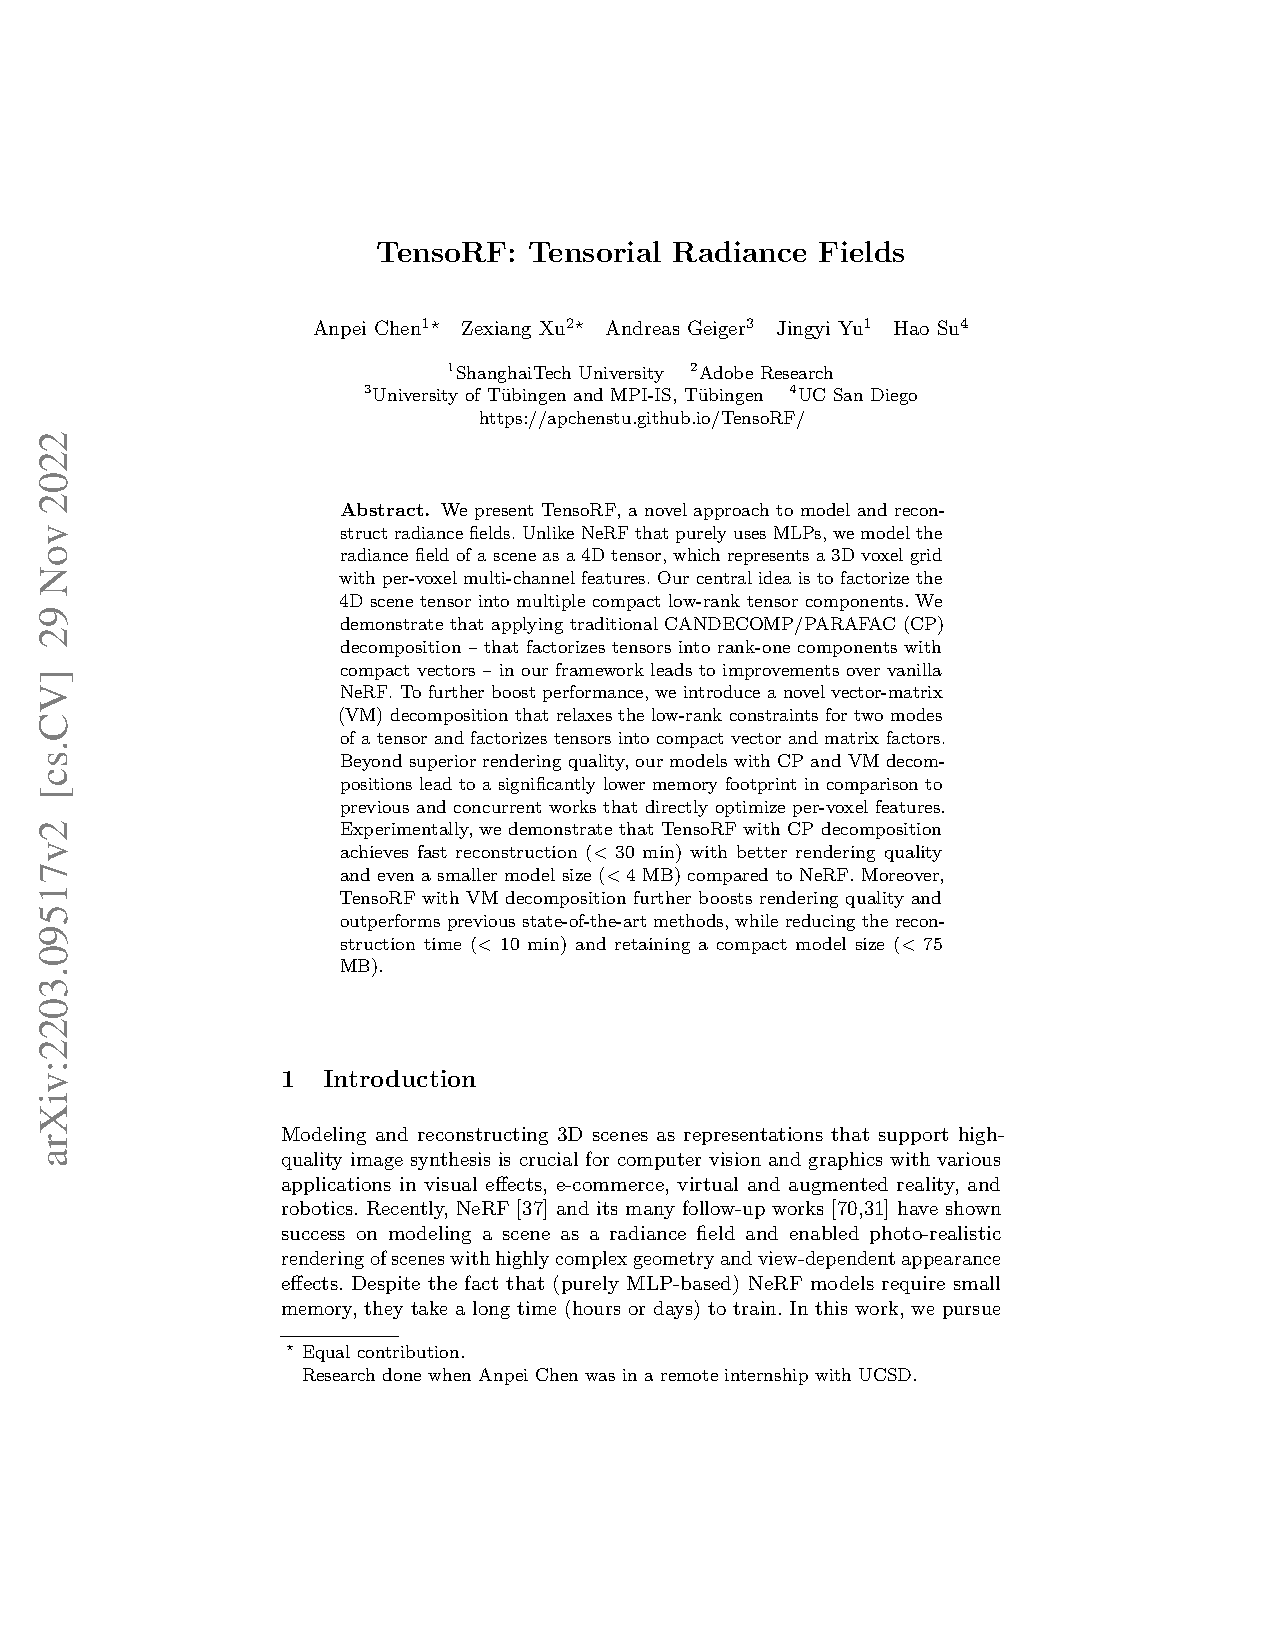
\includegraphics[width=0.9\linewidth]{img/TensoRF.png}
\caption{pipeline of TensoRF}
\label{TensoRF pipeline}
\end{figure}

The work TensoRF(Tensorial Radiance Fields) \cite{TensoRF} proposed a fast training method that does not require a large amount of storage space, comparable to SOTA in rendering quality.

The pipeline of TensoRF could be seen in figure \ref{TensoRF pipeline}.

The vanilla NeRF is based on the coordinates, which uses voxel grid. This requires a large GPU memory to store them, increase in the space complexity of $O(n^3)$, $n$ is the scenario's size.

The key idea is to use a Vector Matrix (VM) decomposition algorithm. Using fewer component tensors to represent a scene and rendering images faster and better. The vanilla NeRF did not effectively use the voxel grid, so each feature grid could be seen as a $4$ dimension tensor. The first $3$ dimension is the space coordinate $x,y,z$, and the $4$-th dimension is the feature. Then the decomposition algorithm could be used greatly reduced to memory consumption. And it has universality and can be innovated using various tensor decomposition algorithms.

The pipeline figure \ref{TensoRF pipeline} shows that the neural radiance field expressed as a set of vectors $v$ and matrix $M$, calculate the volume density and color from this. For each spatial coordinate, we use linear or bilinear sampled values to simulate trilinear interpolation. Add up the volume density along the rays to obtain a density value of $A_{\sigma}$. Stack the color values together to obtain a vector, then multiply it with the appearance matrix $B$, and use the decoding function $S$ to obtain the color $c$.

So we can see that the TensoRF could greatly improve the training efficiency of of the NeRF's process. 

% --------------------------------
\subsection{Instant-NGP}
\label{instant ngp paper reading}

\begin{figure}[htbp]
\centering
\includegraphics[width=0.9\linewidth]{img/hash_encoder.png}
\caption{hash encoder}
\label{hash encoder}
\end{figure}

The work Instant-NGP(Instant Neural Graphics Primitives) \cite{instant-ngp} proposed a way that with hash encoding in figure \ref{hash encoder}. It firstly converts the coordinate $(x,y,z)$ into the index of the hash table. And the different resolution level has different results(red and blue in the figure). Then do the tri-linear interpolation, concat the result vectors as the feature vector. Then the feature vector is sent to the neural network. 

The Instant-NGP mainly used $2$ MLP, one is similar to the vanilla NeRF,  the density feature encoding at multiple resolutions corresponding to the sampling point is output by the multi solution hash encoding, mixed according to different weights, and decoded to obtain the true density value.

Compared dimensions of MLP in NGP and the number of layers in the network is also much smaller than the vanilla NeRF. This makes Instant-NGP run much faster than the vinalla NeRF.

% --------------------------------
\subsection{Nerfstudio}
The work Nerfstudio \cite{nerfstudio} proposed an integration work, it integrate various NeRF technologies into reusable modular components. And it did real time visualization of NeRF scenes through rich controls. Which makes users much easier to use the tools and the pipeline.
\section{Task1: Implementation of NeRF accelerate method}
\label{sec:intro}

We took $3$ videos in different scenarios, then we can implement the dataloader of them, and put them into the vinilla NeRF, the NGP, and the TensoRF. Then we could compare the difference among them.

% --------------------------------
\subsection{Scenarios}
\label{scenarios}

To make the testing diverse, the scenarios were taken indoor and outdoor, big and small.

The scenario $1$ is a small object stationery.

The scenario $2$ is a bigger object chair.

The scenario $3$ is also a chair, but with matting preparation in order to chase for a better behavior. The code part for the matting can be seen in to folder '\textit{matting tool'}. 

The $3$ scenarios look like in figure \ref{the 3 scenarios}. From left to right are scenario $1$, scenario $2$, scenario $3$ respectively.

\begin{figure}[htbp]
	\centering
	\includegraphics[width=0.32\linewidth]{result/scenario/scenario1.png}
	\includegraphics[width=0.32\linewidth]{result/scenario/scenario2.png}
	\includegraphics[width=0.32\linewidth]{result/scenario/scenario3.png}
 \caption{the $3$ scenarios}
	\label{the 3 scenarios}
\end{figure}

% --------------------------------
\subsection{dataloader}
\label{data loader}

Since we took the videos of the $3$ scenarios, but the NeRFs' input should be the images and the intrinsic parameters of the cameras.

With the help of the nerfstudio's integration, and the usage of colmap, we can input the video, and generate the internal and external parameters of cameras. Which is exactly the input for NeRF.

And the frames of the videos were split into the training dataset, validation dataset, and the testing dataset. Each dataset include the images and the correspondence cameras' intrinsic parameters.

Then with the prepared datasets, we could implement the methods in different scenarios.

%  --------------------------------
\subsection{metrics}
\label{metric}
The training information training time(minute:second),  GPU memory consumption(MB), and the training  metrics are PSNR, SSIM, LPIPS. The methods' metrics comparison are shown in the section \ref{conclusion}.

Where PSNR, SSIM and LPIPS are metrics to evaluate image quality.

- PSNR(Peak Signal-to-Noise Ratio) is defined as:
$$\text{PSNR}=10\cdot \log_{10}\dfrac{\text{MAX}_I^2}{\text{MSE}}$$
Where $\text{MAX}_I$ is the max value of the pixels in image $I$, and the MSE of two images $I,K$ is:
$$\text{MSE}=\dfrac{1}{mn}\sum_{i=0}^{m-1}\sum_{i=0}^{n-1}\|I(i,j)-K(i,j)\|^2$$

- SSIM(Structural Similarity Index Measure) is used for comparing the similarity of two images from $3$ key features: Luminance, Contrast, and Structure.

1. Luminance is the average gray scale measurement, obtained by averaging the values of all pixels. Defined as:
$$\mu_x=\frac{1}{N} \sum_{i=1}^N x_i$$
And its contrast function is:
$$l(x, y)=\frac{2 \mu_x \mu_y+C_1}{\mu_x^2+\mu_y^2+C_1}$$

2. Contrast is easured by the grayscale standard deviation. Unbiased estimation of standard deviation:
$$\sigma_x=\left(\frac{1}{N-1} \sum_{i=1}^N\left(x_i-\mu_x\right)^2\right)^{\frac{1}{2}}$$

And its contrast function is:
$$c(x, y)=\frac{2 \sigma_z \sigma_y+C_2}{\sigma_z^2+\sigma_y^2+C_2}$$

3. Structure is the comparison is made after normalization $x-\dfrac{\mu_x}{\sigma_x}$ and $\dfrac{y-\mu_y}{\sigma_y}$, i.e. can be measured by correlation coefficient:

$$s(x, y)=\frac{\sigma_{x y}+C_3}{\sigma_x \sigma_y+C_3}$$
$$\sigma_{x y}=\frac{1}{N-1} \sum_{i=1}^N\left(x_i-\mu_x\right)\left(y_i-\mu_y\right)$$

So SSIM is the combination of Luminance, Contrast, and Structure:
$$\text{SSIM}(x, y)=l(x, y)^\alpha \cdot c(x, y)^\beta \cdot s(x, y)^\gamma$$
Where $\alpha, \beta, \gamma$ is the ratio of each of the $3$ parts of the features.

- LPIPS(Learned Perceptual Image Patch Similarity)  is an indicator for measuring image similarity. It learns an image similarity measurement method through deep learning that can better simulate the human visual system.  The lower it is, the two images are more likely to be the same.
\section{Task2: Processing of our own $3$ scenarios of the accelerate methods}

We can implement the accelerate methods(NGP, TensoRF) on $3$ scenarios, which were introduced in \ref{scenarios}.

With the dataloader \ref{data loader}, we can use our own scenarios to run the accelerate methods and test the behaviors.

The vanilla NeRF without any acceleration \cite{nerf_pytorch} were also implemented as the baseline to compare with.

% --------------------------------
\subsection{basic settings}
\label{basic settings}

All the code were run under the environment of python3.10.

For the training mode of vanilla-NeRF and TensoRF, we choose the blender mode, and modify the correspondence dataloader.

Since our dataset is somehow bigger than the default once, so the scale should be modify by timing $4$, i.e. the parameter '\textit{aabb\_scale}' is set to be $4$, the '\textit{scene\_box}' is modifed from $[-1.5,-1.5,-1.5],[1.5,1.5,1.5]$ to $[-6,-6,-6],[6,6,6]$.

The training iterations for the vanilla NeRF, TensoRF, NGP, and the improvement method are all set to be default iterations. 

And other settings are by default.

% --------------------------------
\subsection{way to run the code}
\label{way to run code}

To run the code and see the results, the details are in the jupyter notebook \textit{NeRF.ipynb}, just run all modules in it would work. The running records are all in \textit{NeRF.ipynb}.

% --------------------------------
\subsection{results}
\begin{figure*}
\includegraphics[width=0.9\textwidth]{result/result.png} 
\caption{novel synthesis view of the $3$ scenarios}
\label{result}
\end{figure*}

The running records are all in \textit{NeRF.ipynb}.

The metrics mentioned in \ref{metric} would be shown in section \ref{conclusion}. And the figures \ref{result} are one of the results of the novel synthesis view of the $3$ scenarios.

Since the dataset are seperated into training, testing, validation dataset. So all the novel synthesis view of the $3$ scenarios are chosen from the testing dataset, so the novel view exist ground truth for comparison.
\section{Task3: Improve the performance by reasonably combining NGP and TensoRF}

We can merge the accelaration methods such as TensoRF and the Instant-NGP, take the advantages of them in order to chase a better performance. Such as a faster training time, or lower memory consuption, or better behavior(the metrics PSNR, SSIM, LPIPS, etc.).

% --------------------------------
\subsection{implement method}

Since TensoRF is implementing VM decomposing algorithm to decompose tensors, and Instant-NGP with hash encoding also generate a feature, with could be seen as a tensor. So with such inspiration, we can try to add method to decompose feature vector that were generated by Instant-NGP with VM mentioned in TensoRF.

Due to the time limit, the method were implemented with a naive implement, it may include much bugs or parameters to adjustment to achieve better performance.

% --------------------------------
\subsection{basic settings and way to run code}
Since the improved method was implemented on the base of Instant-NGP, so all settings were same with the previous work \ref{basic settings}. And to run the code, it is in the same jupyter notebook mentioned in \ref{way to run code}. Just run the module of the \textit{improved method} would work.

% --------------------------------
\subsection{results}

The result images were also shown in figure \ref{result}. And the training time, memory usage, metrics(PSNR, SSIM, LPIPS) were also shown in the table of section \ref{conclusion}.
\section{conclusion}
\label{conclusion}
From the implements above, we can compare the accelerate effect of the vanilla NeRF, tensoRF, and NGP.

All the tasks' experiments were down in the following  hardware configuration:\\
GPU:NVIDIA GeForce RTX 4090.\\
CPU: 13th Gen Inter(R) Core(TM) i9-13900KF of 32 cores.

And the comparison of different methods in the different scenarios are in the following tables, we could discover that the both TensoRF and Instant-NGP has the better performance in acceleration. Which is much faster than the Vanilla NeRF.

The Instant-NGP has the lowest training time, and TensoRF has the lowest rendering time, the different implement methods has their own advantages. The rendering result for the different method is close, and perhaps the vanilla-NeRF requires more training times, so it is worse than others.

Since the background are the noise, so for the scenario $1$ and scenario $2$, we can see some foggy blur in the images, and the performance metrics are lower. With the help of matting the images, the model will not be effected by the background noise, so we can see the scenario $3$ has better performance, and has much less foggy blur.

For the our method trying to improve effects, we tried to merge the advantages of the Instant-NGP and TensoRF method by applying VM decomposing to the hash encoded feature tensor. Since it was modified based on Instant-NGP, so their metrics are close.

There may be further methods under exploration, but due to the time limitation, the effect achieved by us was not quite well, there are much more things need to learn, and lots of experiments need to do, which attract us to put more effort in later studying and researching. Hope we could learn more and chase for better performance. 

% ---------------------------------------------------------------
% Scenario 1
\begin{table}[htbp]
\centering
\begin{tabular}{|c|c|c|c|c|c|c|}
\hline Method &training time$\downarrow$ & rendering time$\downarrow$  & Size$\downarrow$ & PSNR$\uparrow$ & SSIM$\uparrow$ & LPIPS$\downarrow$ \\
\hline vanilla NeRF\cite{nerf_pytorch} & 317:26 & --- &  10874 & 27.825 & 0.784 & 0.308 \\
\hline TensoRF\cite{TensoRF} & 69:10  & 103:39 & \textbf{8255} & 31.422 & \textbf{0.897} & 0.215 \\
\hline NGP\cite{instant-ngp} & \textbf{5:12} & \textbf{55:19} & 11031 & 30.99 & 0.83 & \textbf{0.174}\\
\hline our method & 6:18 & 65:21 & 12063 & \textbf{31.493} & 0.886 & 0.195 \\
\hline
\end{tabular}
\caption{Scenario 1}
\label{Scenario 1}
\end{table}

% ---------------------------------------------------------------
% Scenario 2
\begin{table}[htbp]
\centering
\begin{tabular}{|c|c|c|c|c|c|c|}
\hline Method & training time$\downarrow$ & rendering time$\downarrow$ & Size$\downarrow$ & PSNR$\uparrow$ & SSIM$\uparrow$ & LPIPS$\downarrow$  \\
\hline vanilla NeRF\cite{nerf_pytorch} & 279:19  & --- & 5422 & 31.13 & 0.902 & 0.174 \\
\hline TensoRF\cite{TensoRF} & 70:51 &  60:29  & 15376 & 35.319 & 0.938 & \textbf{0.043} \\
\hline NGP\cite{instant-ngp} & 5:20 & \textbf{40:44} & \textbf{2630} & \textbf{36.54} & 0.893 & 0.112 \\
\hline our method & \textbf{5:00} & 67:46 & 7625 & 35.896 & \textbf{0.943} & 0.138 \\
\hline
\end{tabular}
\caption{Scenario 2}
\label{Scenario 2}
\end{table}

% ---------------------------------------------------------------
% Scenario 3
\begin{table}[htbp]
\centering
\begin{tabular}{|c|c|c|c|c|c|c|}
\hline Method & training time$\downarrow$ & rendering time$\downarrow$  & Size$\downarrow$ & PSNR$\uparrow$ & SSIM$\uparrow$ & LPIPS$\downarrow$  \\
\hline vanilla NeRF\cite{nerf_pytorch} & 303:49 & --- & 5445 & 32.518 & 0.914 & 0.128  \\
\hline TensoRF\cite{TensoRF} & 77:12  & \textbf{10:27} & 5910 & \textbf{37.876} & 0.941 & \textbf{0.022}  \\
\hline NGP\cite{instant-ngp} & 4:31  & 79:13 & \textbf{2689} & 37.561 & \textbf{0.955} & 0.057 \\
\hline our method & \textbf{3:33} & 45:26 & 6913 & 37.642 & 0.944  & 0.042  \\
\hline
\end{tabular}
\caption{Scenario 3}
\label{Scenario 3}
\end{table}
{
    \small
    \bibliographystyle{ieeenat_fullname}
    \bibliography{main}
}

% WARNING: do not forget to delete the supplementary pages from your submission 
% \input{sec/X_suppl}

\end{document}
